%%%%%%%%%%%%%%%%%%%%%%%%%%%%%%%%%%%%%%%%%
% Structured General Purpose Assignment
% LaTeX Template
%
% This template has been downloaded from:
% http://www.latextemplates.com
%
% Original author:
% Ted Pavlic (http://www.tedpavlic.com)
%
% Note:
% The \lipsum[#] commands throughout this template generate dummy text
% to fill the template out. These commands should all be removed when 
% writing assignment content.mus
%
%%%%%%%%%%%%%%%%%%%%%%%%%%%%%%%%%%%%%%%%%

%----------------------------------------------------------------------------------------
%	PACKAGES AND OTHER DOCUMENT CONFIGURATIONS
%----------------------------------------------------------------------------------------

\documentclass{article}

\usepackage[brazilian]{babel}
\usepackage[utf8]{inputenc}
\usepackage{fancyhdr} % Required for custom headers
\usepackage{lastpage} % Required to determine the last page for the footer
\usepackage{extramarks} % Required for headers and footers
\usepackage{graphicx} % Required to insert images
\usepackage{float}
\usepackage{listings}
\usepackage[colorlinks=true, pdfborder={0 0 0}, urlcolor=blue, linkcolor=black]{hyperref}

\graphicspath{ {img/} }

% Margins
\topmargin=-0.45in
\evensidemargin=0in
\oddsidemargin=0in
\textwidth=6.5in
\textheight=9.0in
\headsep=0.25in 

\linespread{1.1} % Line spacing

% Set up the header and footer
\pagestyle{fancy}
\lhead{\hmwkAuthorName} % Top left header
%\chead{\hmwkClass\ (\hmwkClassInstructor\ \hmwkClassTime): \hmwkTitle} % Top center header
\rhead{\hmwkClass: \hmwkTitle} % Top center header
%\rhead{\firstxmark} % Top right header
\lfoot{\lastxmark} % Bottom left footer
\cfoot{} % Bottom center footer
\rfoot{Página\ \thepage\ de\ \pageref{LastPage}} % Bottom right footer
\renewcommand\headrulewidth{0.4pt} % Size of the header rule
\renewcommand\footrulewidth{0.4pt} % Size of the footer rule

\setlength\parindent{0pt} % Removes all indentation from paragraphs

%----------------------------------------------------------------------------------------
%	DOCUMENT STRUCTURE COMMANDS
%	Skip this unless you know what you're doing
%----------------------------------------------------------------------------------------

% Header and footer for when a page split occurs within a problem environment
\newcommand{\enterProblemHeader}[1]{
\nobreak\extramarks{#1}{#1 continuação na próxima página\ldots}\nobreak
\nobreak\extramarks{#1 (continuação)}{#1 continuação na próxima página\ldots}\nobreak
}

% Header and footer for when a page split occurs between problem environments
\newcommand{\exitProblemHeader}[1]{
\nobreak\extramarks{#1 (continuação)}{#1 continuação na próxima página\ldots}\nobreak
\nobreak\extramarks{#1}{}\nobreak
}

\setcounter{secnumdepth}{0} % Removes default section numbers
\newcounter{homeworkProblemCounter} % Creates a counter to keep track of the number of problems

\newcommand{\homeworkProblemName}{}
\newenvironment{homeworkProblem}[1][Questão \arabic{homeworkProblemCounter}]{ % Makes a new environment called homeworkProblem which takes 1 argument (custom name) but the default is "Problem #"
\stepcounter{homeworkProblemCounter} % Increase counter for number of problems
\renewcommand{\homeworkProblemName}{#1} % Assign \homeworkProblemName the name of the problem
\section{\homeworkProblemName} % Make a section in the document with the custom problem count
\enterProblemHeader{\homeworkProblemName} % Header and footer within the environment
}{
\exitProblemHeader{\homeworkProblemName} % Header and footer after the environment
}

\newcommand{\problemAnswer}[1]{ % Defines the problem answer command with the content as the only argument
\noindent\framebox[\columnwidth][c]{\begin{minipage}{0.98\columnwidth}#1\end{minipage}} % Makes the box around the problem answer and puts the content inside
}

\newcommand{\homeworkSectionName}{}
\newenvironment{homeworkSection}[1]{ % New environment for sections within homework problems, takes 1 argument - the name of the section
\renewcommand{\homeworkSectionName}{#1} % Assign \homeworkSectionName to the name of the section from the environment argumen
\subsection{\homeworkSectionName} % Make a subsection with the custom name of the subsection
\enterProblemHeader{\homeworkProblemName\ [\homeworkSectionName]} % Header and footer within the environment
}{
\enterProblemHeader{\homeworkProblemName} % Header and footer after the environment
}
   
%----------------------------------------------------------------------------------------
%	NAME AND CLASS SECTION
%----------------------------------------------------------------------------------------

\newcommand{\hmwkTitle}{Trabalho Final} % Assignment title
\newcommand{\hmwkDueDate}{01 de julho de 2014} % Due date
\newcommand{\hmwkClass}{INF01047} % Course/class
\newcommand{\hmwkClassFull}{INF01047: Fundamentos de Computação Gráfica} % Course/class
\newcommand{\hmwkClassTime}{} % Class/lecture time
\newcommand{\hmwkClassInstructor}{} % Teacher/lecturer
\newcommand{\hmwkAuthorName}{Fernando Bombardelli da Silva(218324), William Bombardelli da Silva(218323)} % Your name

%----------------------------------------------------------------------------------------
%	TITLE PAGE
%----------------------------------------------------------------------------------------

\title{
%\vspace{2in}
\Large\textmd{\textbf{\hmwkClassFull}}\\
\normalsize{\textbf{\hmwkTitle}}\\
\normalsize\vspace{0.1in}\small{\hmwkDueDate}\\
%\vspace{0.1in}
\large{\textit{\hmwkClassInstructor\ \hmwkClassTime}}
%\vspace{3in}
}

\author{\textbf{\hmwkAuthorName}}
\date{} % Insert date here if you want it to appear below your name

%----------------------------------------------------------------------------------------

\begin{document}

%\maketitle
{\centering
\Large\textmd{\textbf{\hmwkClassFull}}\\
\normalsize{\textbf{\hmwkTitle}}\\
\normalsize\vspace{0.1in}\small{\hmwkDueDate}\\
%\vspace{0.1in}
\large\textbf{\hmwkAuthorName}
%\large{\textit{\hmwkClassInstructor\ \hmwkClassTime}}\\

}
%----------------------------------------------------------------------------------------
%	TABLE OF CONTENTS
%----------------------------------------------------------------------------------------

%\setcounter{tocdepth}{1} % Uncomment this line if you don't want subsections listed in the ToC

%\newpage
%\tableofcontents
%\newpage

% To have just one problem per page, simply put a \clearpage after each problem

%----------------------------------------------------------------------------------------
%	Questão 1
%----------------------------------------------------------------------------------------

\begin{homeworkProblem}[Relatório de desenvolvimento]
Nesse documento relatamos brevemente o desenvolvimento do trabalho final da disciplina de Fundamentos de Computação Gráfica. Basicamente, foi desenvolvido um jogo de título \textbf{Pengo}, onde o jogador é o personagem principal (um pinguim), que está em uma mapa com blocos de gelo. Seu objetivo é matar todos os seus inimigos (as abelhas \emph{snowbees}) por deslizar os blocos de gelo em direção à elas. O fim do jogo se dá caso \emph{Pengo} mate todos os inimigos (nesse caso há a vitória do jogador), ou algum dos inimigos entre em contato com \emph{Pengo} (derrota do jogador). O \emph{game} foi desenvolvido para Linux na linguagem C++ com o uso de OpenGL.

Em relação aos requisitos do trabalho, todos foram cumpridos com sucesso, desde o carregamento do cenário com os objetos e texturas até a inteligência artificial básica dos inimigos. A única exceção foi quanto à entrada do comando \emph{Shift} do teclado, o qual a \emph{GLUT toolkit} é incapaz de tratar como um \emph{key press} isolado. Como alternativa ao problema, utilizamos a tecla \emph{E} para o comando de criação de blocos móveis. Alternativamente, poderíamos capturar o evento dessa tecla diretamente no sistema operacional, porém acreditamos que ficaria fora do escopo e objetivos propostos no trabalho.

Sobre o mapa, implementamos um de 16x16 posições, que é definido na inicialização do jogo a partir do arquivo de imagem com nome \emph{map.bmp} na pasta \emph{res} e formato \emph{Bitmap} de 24 \emph{bits} por \emph{pixel}. Convenção de cores:
\begin{itemize}
\item Vermelho (RGB(1,0,0)) para bloco imóvel;
\item Verde (RGB(0,1,0)) para bloco móvel.
\end{itemize}

\begin{figure}[H]
\centering
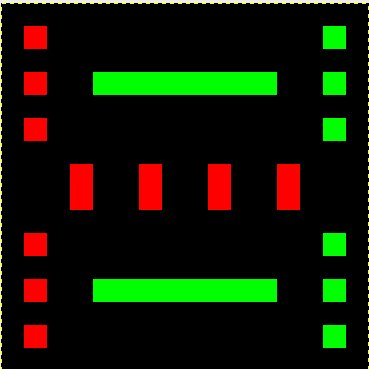
\includegraphics[scale=0.5]{map_large}
\caption{\label{fig:map_large}Exemplo de Imagem de Mapa}
\end{figure}

A posição do \emph{Pengo}, dos inimigos e dos itens dentro de blocos é definido randomicamente na inicialização do mapa.
\end{homeworkProblem}

\begin{homeworkProblem}[Principais Problemas Encontrados]

Entre os problemas encontrados no desenvolvimento do trabalho podemos citar principalmente três:
\begin{itemize}
\item As bibliotecas utilizadas para carregamento de modelos e texturas não são robustas, tampouco são à prova de falhas, além de mal documentadas;
\item Há dificuldade de se encontrar na web bons modelos 3D no formato \emph{OBJ} com texturas;
\item O desenvolvimento em C++ reduz muito a produtividade do programador, que precisa se preocupar em gerenciar memória, além de despender muito tempo para \emph{debug}.
\end{itemize}

Portanto, no contexto do desenvolvimento de jogos com computação gráfica, podemos ver claramente a necessidade de uma equipe de arte que gere bons modelos, além de programadores com experiência em C++ e OpenGL ou da utilização de uma linguagem e uma API gráfica mais produtivas.
\end{homeworkProblem}

\end{document}

